\documentclass[a4paper,11pt,normalheadings,idxtotoc,bibtotoc,headsepline]{scrbook} % bibtotocnumbered, chapterprefix
%\linespread{1.2}
%\usepackage{typearea}
%\areaset[0cm]{16cm}{26cm}
\usepackage{scrpage2}
\renewcommand{\headfont}{%
\normalfont\sffamily\bfseries\color[rgb]{0 0 1}
}
\renewcommand{\pnumfont}{%
\normalfont\rmfamily\slshape\color[rgb]{0 0 0}
}
\usepackage{pstricks}
\usepackage{graphicx}
\usepackage{multicol}
\usepackage[T1]{fontenc}
\usepackage{makeidx}
\makeindex
%\usepackage[bitstream-charter]{mathdesign}
%\usepackage{fourier}
%\usepackage{lmodern}
\usepackage{amsmath}
\usepackage{textcomp}
%\usepackage{pxfonts}
\usepackage{lmodern}
\renewcommand{\rmdefault}{ugm}
%\usepackage{courier}
%\usepackage{kpfonts}
%\usepackage{helvet}
%\usepackage{mathptmx}
%\usepackage{mathpazo}
%\usepackage{times}
\usepackage{microtype}
\usepackage{jneurosci}
\usepackage[greek,german,english]{babel}
\bibliographystyle{jneurosci}
\usepackage{amssymb}

\usepackage[colorlinks=true,linkcolor=black,citecolor=black,urlcolor=black]{hyperref}

\usepackage{listings}
\lstset{ language=Python }
\lstset{
    basicstyle=\ttfamily,
    keywordstyle=\color{blue}\bfseries,
    commentstyle=\color{red}\itshape,
    stringstyle=\color{violet},
    showstringspaces=false,
    numbers=none,
    numberstyle=\tiny\sffamily,
    stepnumber=1,
    numbersep=10pt
}
\usepackage[labelfont=sf,bf]{caption}

\usepackage{float}
\usepackage{floatflt}
\newfloat{listing}{htb}{}   % optional numbering with [section] or [chapter]
\floatname{listing}{Listing}

\newfloat{myfigure}{htb}{}
\floatname{myfigure}{Fig.}

\setkomafont{chapter}{\LARGE \color[rgb]{0 0 1}}
% \setkomafont{captionlabel}{\bfseries \sffamily \small}
% \setkomafont{caption}{\small}
% \setcapindent{0cm}

\setlength{\marginparsep}{3mm}
\setlength{\marginparwidth}{3.53cm}

\newcommand\keybox[1]{\psframebox[framesep=1.5pt,framearc=0.3]{\centering\sffamily{#1}}}
\newcommand\marginkey[1]{\marginline{\small{\textit{#1}}}}
\newcommand\marginpy[1]{\marginline{\scriptsize\textcolor{blue}{\texttt{#1}}}}
\newcommand\infobox[1]{%
  \noindent\psframebox{%
    \begin{minipage}[t]{0.975\textwidth}%
    \textcolor[rgb]{0 0.5 0}{\textbf{Note:} #1}%
    \end{minipage}%
  }}
\newcommand\pycommand[1]{\texttt{#1}}
\newcommand\pyindex[2]{\label{#1}\index{Python functions!\texttt{#2}}\marginpy{#2}}
\newcommand\pyindexonly[2]{\label{#1}\index{Python functions!\texttt{#2}}}
\newcommand\keyindex[3]{\label{#1}\index{#2}\marginkey{#3}}


% Title Page
\title{stimfit manual\\\normalsize rev. 0.8.13.1}
\author{Christoph Schmidt-Hieber}
\date{\today}

\begin{document}
\pagestyle{scrheadings}

\frontmatter

\maketitle

\tableofcontents

\chapter{Preface}

Stimfit was originally written by Peter Jonas, University of Freiburg, in the early 1990s. It was primarily designed to analyse the kinetics of evoked excitatory postsynaptic currents (EPSCs; \citetext{Jonas93}). The name ``Stimfit'' was chosen because the program allowed to \textit{fit} exponential functions to the decay of EPSCs evoked by extracellular \textit{stim}ulation\footnote{Be reassured that I would choose a different name if I had to sell the program.}. The program was written in Borland Pascal, running under DOS and entirely controlled using keyboard shortcuts (Fig. \ref{stimfitdos}). The user interface was similar to a digital oscilloscope, with vertical cursors defining measurement windows for baseline calculation, peak detection and curve fitting. This allowed to analyse data with surprising efficiency once the keyboard shortcuts were mastered. However, the Borland Pascal compiler imposed some significant restrictions which became apparent with increasing data size and computing power: for instance, arrays were not allowed to be longer than 10\textsuperscript{4} elements, and faster processors had to be artificially slowed down to avoid runtime errors.
\begin{myfigure}[ht]
    \begin{center}
      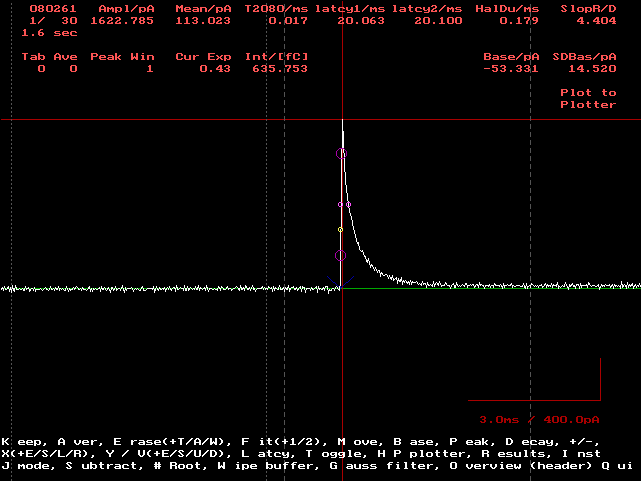
\includegraphics[scale = 0.5]{./img/stimfit_dos.eps}
    \end{center}
    \caption{The original Stimfit for DOS.}
    \label{stimfitdos}
\end{myfigure}

When I converted the original Pascal program to C/C++, I rewrote the code almost entirely from scratch. Only the algorithms to calculate latencies, rise times, half durations and slopes are direct translations of the original Pascal code. By contrast, I tried to preserve the user interface as far as possible. Therefore, the program only poorly adheres to common conventions for graphical user interfaces: For instance, clicking the right mouse button will usually set a cursor position rather than popping up a context menu.

A number of people have contributed to the program: First, I would like to thank Peter Jonas for the original Stimfit code. Josef Bischofberger has added some functions to the DOS version which I have adopted. Bill Anderson has made helpful suggestions concerning the user interface and provided some very large files that have been recorded with his free program \href{http://www.winltp.com}{WinLTP}\footnote{\url{http://www.winltp.com}}. A large amount of helpful comments and bug reports were filed by Emmanuel Eggermann and Daniel Doischer. The Levenberg-Marquardt algorithm used for curve fitting was implemented by  \href{http://www.ics.forth.gr/~lourakis/levmar/}{Manolis Lourakis}\footnote{\url{http://www.ics.forth.gr/~lourakis/levmar/}}.


\mainmatter

\chapter{Getting started}

\label{gettingstarted}
\section{File opening}
This tutorial will cover the basic program functionality from opening a file to fitting functions to data.
\begin{itemize}
  \item \href{http://www.stimfit.org/index.php?option=com_content&task=section&id=5&Itemid=27}{Download the Stimfit setup program}\footnote{\url{http://www.stimfit.org}} and install Stimfit on your computer.
  \item \href{http://stimfit.org/tutorial/sample.dat}{Download the sample data file}\footnote{\url{http://stimfit.org/tutorial/sample.dat}}.
  \item Open the data file: you can either double-click it from an Explorer Window, or you can start Stimfit and choose ``File'' $\rightarrow$``Open...'' from the menu.
  \item The file will be opened in a new child window, and the first trace will be displayed.
\end{itemize}

\section{Trace scaling}
\begin{itemize}
  \item If you just see scale bars, but no trace is displayed, press \keybox{F} or click the corresponding button (Fig. \ref{fittowindow}). This will fit the first trace of the active channel (plotted in black) to the screen.
  \begin{myfigure}[htb]
    \begin{center}
      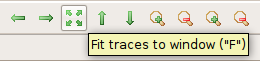
\includegraphics[scale=0.75]{./img/fittowindow.eps}
    \end{center}
    \caption{Fit traces to the window size.}
    \label{fittowindow}
  \end{myfigure}
  \item If you prefer coordinates to scale bars, you can uncheck ``View''$\rightarrow$``Scale bars'' in the menu (Fig. \ref{viewscalebars}).
  \begin{myfigure}[ht]
    \begin{center}
      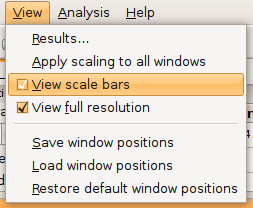
\includegraphics[scale=0.5]{./img/viewscalebars.eps}
    \end{center}
    \caption{Show coordinates rather than scale bars.}
    \label{viewscalebars}
  \end{myfigure}
  \item Fit the inactive channel (plotted in red) to the screen as well: Press \keybox{3}. The buttons labelled ``1'' and ``2'' should now both be highlighted (Fig. \ref{channelselection}). That means that any changes to the scaling will now be applied to both channels simultaneously. Press \keybox{F} again. The inactive channel (red trace) will now be fitted to the screen as well. If you want to scale channels individually, press either \keybox{1} or \keybox{2}.
  \begin{myfigure}[ht]
    \begin{center}
      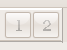
\includegraphics[scale=0.75]{./img/channelselection.eps}
    \end{center}
    \caption{Scaling applies to both channels.}
    \label{channelselection}
  \end{myfigure}
  \item Enlarge the vertical scale: Press \keybox{+}. Depending on which channel(s) you selected, the vertical scale will be enlarged by a factor of 10\%. Shrink the scale back to its original value by pressing \keybox{-}.
  \item Enlarge the time scale: Press \keybox{Ctrl} and \keybox{+} simultaneously. The time scale will be enlarged for both channels, regardless of which channel you have chosen, because Stimfit assumes that both channels have been sampled at the same time and frequency.
  \item Shrink the time scale back to its original value by pressing \keybox{Ctrl} and \keybox{-} simultaneously.
  \item Shift the trace by pressing \keybox{Ctrl} and one of the cursor (arrow) keys simultaneously.
  \item You can zoom into parts of the trace using a zoom window: Press \keybox{Z}. The zoom button (showing a magnifying glass) will be highlighted (Fig. \ref{zoom}).
  \begin{myfigure}[ht]
    \begin{center}
      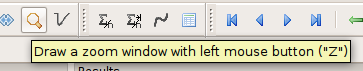
\includegraphics[scale=0.5]{./img/zoom.eps}
    \end{center}
    \caption{Setting the mouse cursor to draw zoom windows.}
    \label{zoom}
  \end{myfigure}
  \item Drag a window over the region of interest holding down the left mouse button. Release the left mouse button once you are done. When you right-click on the window, a menu will pop up showing different zoom options. Select ``Expand zoom window horizontally \& vertically'' (Fig. \ref{popupzoom}).
  \begin{myfigure}[ht]
    \begin{center}
      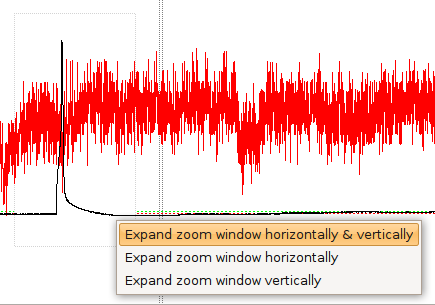
\includegraphics[scale=0.5]{./img/zoompopup.eps}
    \end{center}
    \caption{Magnifying a region of interest.}
    \label{popupzoom}
  \end{myfigure}
  \item If you can't see any trace because you zoomed in or out too much, press \keybox{F} to fit the trace to the screen again.
\end{itemize}
  \infobox{Although all commands mentioned above can be accessed with the mouse, I strongly recommend using the keyboard shortcuts; once you get used to it, the shortcuts are much faster (see p. \pageref{shortcuts} for a list).}

\section{Navigate within a file}
\begin{itemize}
  \item You can toggle through \keyindex{tracesselection}{traces!selection}{traces}traces using the \keybox{$\leftarrow$} or \keybox{$\rightarrow$} keys (\textit{without} pressing \keybox{Ctrl} at the same time). The current trace number will be displayed in the drop-down box labelled "Trace ... of ...". You can directly select a trace from this box as well (Fig. \ref{traceselection}).
  \begin{myfigure}[ht]
    \begin{center}
      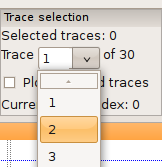
\includegraphics[scale=0.5]{./img/traceselection.eps}
    \end{center}
    \caption{Selecting a trace.}
    \label{traceselection}
  \end{myfigure}
  \item All measurements will be performed on the active channel plotted in black. You can swap \keyindex{channelindex}{channels!selection}{channels}channels by either selecting ``View''$\rightarrow$``Swap channels'' from the menu, or setting the channels in the drop-down boxes (Fig. \ref{channeldrop}).
  \begin{myfigure}[ht]
    \begin{center}
      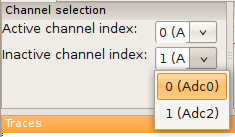
\includegraphics[scale=0.5]{./img/channelselectiondrop.eps}
    \end{center}
    \caption{Setting the active and inactive channel.}
    \label{channeldrop}
  \end{myfigure}
\end{itemize}

\section{Analyse individual events}
An ``event'' can be anything from an EPSC to an action potential. In this case, we will analyse a large spontaneous EPSC in trace no. 12 of the second channel. Navigate to trace number 12, swap channels, and zoom into the large EPSC as described above. All results are displayed in the \keyindex{results}{results table}{results table}results table (Fig. \ref{resultstable}). You can select which results to show in the table by right-clicking on one of the column or row title labels, and then selecting or unselecting the corresponding items.
  \begin{myfigure}[ht]
    \begin{center}
      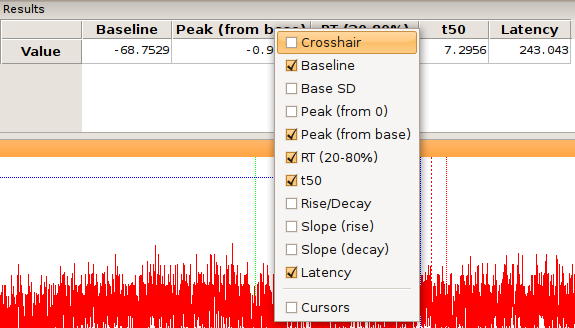
\includegraphics[scale=0.5]{./img/resultstable.eps}
    \end{center}
    \caption{Showing analysis results.}
    \label{resultstable}
  \end{myfigure}

Stimfit uses \keyindex{cursors}{cursors}{cursors}cursors to define measurement windows. Cursors are represented by vertical dashed lines extending throughout the window, similar as on an oscilloscope. For example, the \keyindex{baselineindex}{baseline}{baseline}baseline is calculated as the average of all sampling points between the two base window cursors (vertical green dashed lines). To move the cursors, press \keybox{B}. The corresponding toolbar button will be highlighted. Set the left cursor by clicking the left mouse button where you want the baseline calculation to start. Set the right cursor by clicking the right mouse button where you want the baseline calculation to end. Press \keybox{Enter}. The result of the baseline calculation is displayed in the results table, and the baseline is plotted as a horizontal green dashed line (Fig. \ref{baseline}).
  \begin{myfigure}[ht]
    \begin{center}
      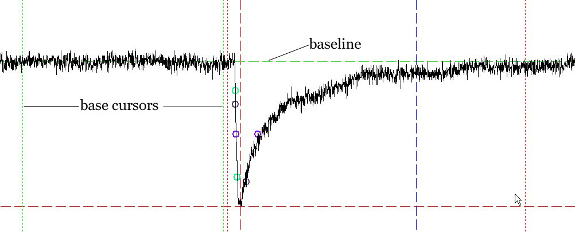
\includegraphics[width=0.7\textwidth]{./img/baseline.eps}
    \end{center}
    \caption{Setting the baseline window cursors.}
    \label{baseline}
  \end{myfigure}
\, \\ \smallskip
\infobox{You have to press \keybox{Enter} after changing any cursor position to update all calculations. Otherwise, you will see the results of your previous cursor settings. Alternatively, you can call \texttt{measure()} from the Python shell (see p. \pageref{measure}).}

The \keyindex{peakcalculation}{peak!calculation}{peak calculation}peak value will be determined between the two peak window cursors (vertical red dashed lines).  To move the cursors, press \keybox{P}. The corresponding toolbar button will be highlighted. Set the left cursor by clicking the left mouse button where you want the peak detection to start. Set the right cursor by clicking the right mouse button where you want the peak detection to end. Press \keybox{Enter}.  The result of the peak calculation is displayed in the results bar. ``Peak (from base)'' is the difference between the peak value and the baseline, and ``Peak (from 0)'' is the ``raw'' value of the peak, measured from zero, without any subtraction. A horizontal red dashed line will indicate the peak value, and a vertical dashed line will indicate the point in time when this peak value has been detected (Fig. \ref{peak}).
  \begin{myfigure}[ht]
    \begin{center}
      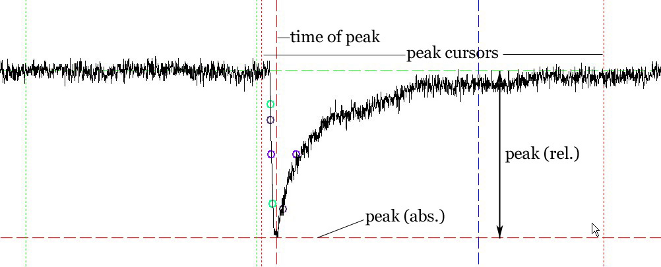
\includegraphics[width=0.7\textwidth]{./img/peak.eps}
    \end{center}
    \caption{Setting the peak window cursors.}
    \label{peak}
  \end{myfigure}

There are three ways the peak value can be calculated: \keyindex{peakdirection}{peak!direction}{peak direction}As a default, it is calculated as the maximal absolute value measured from baseline; hence, both positive- or negative-going events may be detected, whichever is larger. If you want only positive-going events to be detected,  select ``Edit''$\rightarrow$``Cursor settings'' from the menu. A dialog will appear. Select the ``Peak'' tab, and then check the ``Up'' radio button  (Fig. \ref{cursorsettings}). Click the ``Apply'' button to measure the peak using your new settings. If you only want negative-going events to be detected, select ``Down'' instead. Selecting ``Both'' resets the peak calculation to the default mode. If you want to set the peak direction from the Python shell, you can call \pyindex{setpeakdirection}{set\_peak\_direction}\pycommand{set\_peak\_direction(direction)}, where \pycommand{direction} can be one of \pycommand{"up"}, \pycommand{"down"} or \pycommand{"both"}. The Python shell will be explained in some more detail in chapter \ref{pythonshell}.
  \begin{myfigure}[ht]
    \begin{center}
      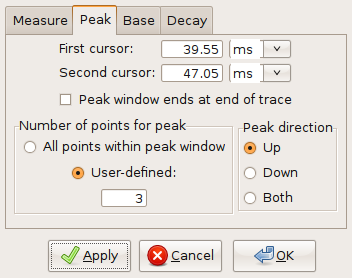
\includegraphics[scale = 0.5]{./img/cursorsettings.eps}
    \end{center}
    \caption{Setting the peak calculation properties.}
    \label{cursorsettings}
  \end{myfigure}

In case the event you want to analyse is noisy, it may be helpful to use the \keyindex{peakmovingaverage}{peak!moving average}{moving average}average of several neighbouring sampling points for the peak calculation instead of a single sampling point. A moving average algorithm will then be used to calculate the peak value. The number of sampling points can either be set in the cursor settings dialog (Fig. \ref{cursorsettings}) or from the Python shell using \pyindex{setpeakmean}{set\_peak\_mean}\pycommand{set\_peak\_mean(pts)}, where \pycommand{pts} is the number of sampling points.

Some other values describing the event can be found in the results table (Fig. \ref{overview}):
\begin{itemize}
  \item \index{rise time}``RT(20-80\%)''refers to the time required for the signal to change from 20 to 80\% of the peak value (measured from baseline), commonly called the ``20-to-80\%-risetime''.  The points corresponding to 20 and 80\% of the peak value are indicated by green circles. They are determined by linear interpolation between neighbouring sampling points.
  \item \index{half duration}``t1/2'' refers to the full width of the signal at half-maximal amplitude (measured from baseline), commonly called "half-duration". The points where the signal reaches its half-maximal amplitude are indicated by blue circles. Again, this is determined by linear interpolation between neighbouring sampling points. 
  \item ``Rise'' and ``Decay'' refer to the maximal slope during the rising and the falling phase of the signal, respectively. The corresponding points are indicated by violet circles.
  \item \index{R/D}``R/D'' is the ratio of the maximal slopes during the rising and the falling phase of the signal.
\end{itemize}

\infobox{From version 0.8.6 on, the rise time and half duration calculation is independent of the baseline and peak window cursor positions. In versions prior to 0.8.6, the baseline cursors had to precede the peak window cursors. However, the calculation of the maximal slopes of rise and decay is still restricted to the peak window.}
  \begin{myfigure}[ht]
    \begin{center}
      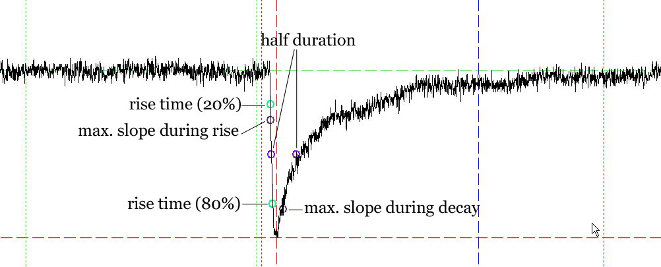
\includegraphics[width=0.7\textwidth]{./img/overview.eps}
    \end{center}
    \caption{Analysis of individual events.}
    \label{overview}
  \end{myfigure}

\section{Average calculation}
First, you have to select the traces that you want to average\keyindex{averagecalculation}{average calculation}{average calculation}: navigate through the file with the \keybox{$\leftarrow$} and \keybox{$\rightarrow$} keys (as described above), and press \keybox{S} if you want to select a trace, or click the selection button. The number of traces that you have already selected will be shown just above the trace selection drop-down box (Fig. \ref{selection}).
  \begin{myfigure}[ht]
    \begin{center}
      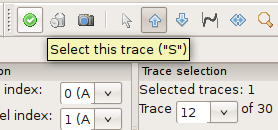
\includegraphics[scale = 0.5]{./img/selection.eps}
    \end{center}
    \caption{Trace selection.}
    \label{selection}
  \end{myfigure}
If you selected a trace accidentally, you can remove it from the selected traces list by pressing \keybox{R} or clicking the trash bin button to the right of the selection button (Fig. \ref{selection}).

Once you are done, click the "Average" button to compute the average of all selected traces (Fig. \ref{average}). A new child window will pop up showing the average. In the original child window, the average is shown as a blue trace.
  \begin{myfigure}[ht]
    \begin{center}
      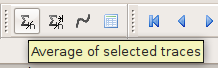
\includegraphics[scale = 0.5]{./img/average.eps}
    \end{center}
    \caption{Average calculation.}
    \label{average}
  \end{myfigure}
\, \\ \smallskip
\infobox{This is a general concept for most analysis functions: you first select traces, and the analysis will then be performed on the selected traces.}

\section{Fitting functions to data}
\index{curve fitting}\index{fitting|see{curve fitting}}\index{nonlinear regression|see{curve fitting}}
\begin{itemize}
\item Navigate to trace number 12 which contains a large spontaneous EPSC. Swap channels as described above, then zoom into the large EPSC.
\item Set the peak and baseline cursors appropriately; the peak and baseline values will be used as initial values for the fit. Don't forget to press \keybox{Enter}.
\item The function will be fitted to the data between the two fit window cursors (grey vertical dashed lines). To move the cursors, press \keybox{D} (historically, ``D'' stands for ``decay''). The corresponding button will be highlighted. Set the left cursor by clicking the left mouse button where you want the fit to start. Set the right cursor by clicking the right mouse button where you want the fit to end. Press \keybox{Enter} to confirm the cursor settings.
\item Select ``Analysis''$\rightarrow$``Fit''$\rightarrow$``Non-linear regression'' from the menu. Select a bi-exponential function (Fig. \ref{fitselection}).
\end{itemize}
  \begin{myfigure}[ht]
    \begin{center}
      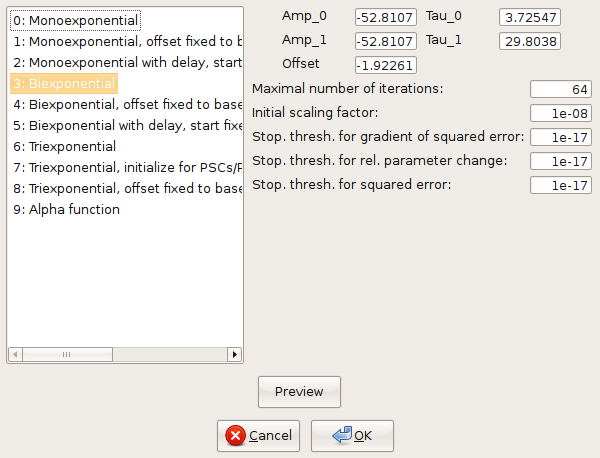
\includegraphics[scale = 0.5]{./img/fitselection.eps}
    \end{center}
    \caption{Non-linear regression settings.}
    \label{fitselection}
  \end{myfigure}
\begin{itemize}
\item The fitted function will be displayed as a thick grey line, and a table showing the best-fit parameters and the sum of squared errors (SSE) will pop up (Fig. \ref{fit}).
\end{itemize}
  \begin{myfigure}[ht]
    \begin{center}
      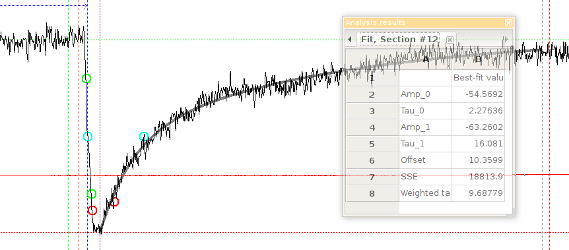
\includegraphics[width=0.7\textwidth]{./img/fit.eps}
    \end{center}
    \caption{Results of a non-linear regression using a bi-exponential function.}
    \label{fit}
  \end{myfigure}
\pycommand{\textbf{leastsq(fselect, refresh=True)}}\pyindex{leastsq}{leastsq}\\ can be called from the Python shell to fit the function with index \pycommand{fselect} to the data. \pycommand{fselect} refers to the number that you can find in front of the functions in the fit settings dialog (see Fig. \ref{fitselection}). If \pycommand{refresh=False}, the trace will not be re-drawn, wich can be useful to avoid flicker when performing a series of fits.

\chapter{The Python shell}

\label{pythonshell}
\section{Before you start}
If you're new to Python, I suggest that you first have a look at the \href{http://docs.python.org/tut/}{Python tutorial}\footnote{\url{http://docs.python.org/tut/}}. If that's not enough, abundant documentation is freely available on the \href{http://www.python.org/doc/}{Python web site}\footnote{\url{http://www.python.org/doc/}}. If you're new to stimfit, I recommend going through the tutorial in chapter \ref{gettingstarted} of this manual first.

\section{The Python shell}
When you start up stimfit, you will find an embedded Python shell in the lower part of the program window. From this shell, you have full access to the Python interpreter. For instance, you could type:
\begin{lstlisting}
>>> stf.
\end{lstlisting}
which will pop up a window showing all the available functions from the stimfit module (abbreviated \pycommand{stf}). For example, you could now check whether a file is open by selecting the \pycommand{check\_doc} \marginpy{check\_doc} function from that list: 
\begin{lstlisting}
>>> stf.check_doc()
False
\end{lstlisting} The function documentation will pop up when you type in the opening bracket. The function returns the boolean value \pycommand{False} because you haven't opened any file yet. Since the \pycommand{stf} module is imported in the namespace, you can omit the initial ``\pycommand{stf.}'' when calling functions. Thus, you could get the same result by simply typing
\begin{lstlisting}
>>> check_doc()
False
\end{lstlisting}
If you press \keybox{Ctrl} and \keybox{$\uparrow$} at the same time, you can go through all the commands that you have previously typed in. This can be very useful when you want to call a function several times in a row.

\section{Accessing data from the Python shell}
\pycommand{\textbf{get\_trace(trace=-1, channel=-1)}}\pyindex{gettrace}{get\_trace}\\
The \pycommand{get\_trace} function returns the currently displayed trace as a one-dimensional \href{http://numpy.scipy.org/}{NumPy}\footnote{\url{http://numpy.scipy.org/}} array when called without any arguments:
\begin{lstlisting}
>>> a = get_trace()
\end{lstlisting}
You can now access individual sampling points using squared brackets to specify the index. For example:
\begin{lstlisting}
>>> print a[123]
-26.3671875
\end{lstlisting}
prints out the y-value of the sampling point with index 123. Note that indices in Python are \textit{zero-based}, i.e. the first sampling point has the index 0:
\begin{lstlisting}
>>> print a[0]
-21.2249755859
\end{lstlisting}
Python will check for indices that are out of range. For example,
\begin{lstlisting}
>>> print a[1e9]
Traceback (most recent call last):
  File "<input>", line 1, in <module>
IndexError: index out of bounds
\end{lstlisting}
You can use the \pycommand{get\_trace(trace=-1, channel=-1)} function to return any trace within a file. The default values of \pycommand{trace = -1} and \pycommand{channel = -1} will return the currently displayed trace of the active channel. By passing a value of 1 as the first argument, you could access the second trace within your file (assuming it contains more than one trace, of course) - remember that indices are zero-based!
\begin{lstlisting}
>>> b = get_trace(1)
>>> print b[234]
-23.7731933594
\end{lstlisting}

\section{Using NumPy with stimfit}
\href{http://numpy.scipy.org/}{NumPy}\footnote{\url{http://numpy.scipy.org/}} allows you to efficiently perform array computations from the Python shell. For example, you can multiply an array with a scalar:
\begin{lstlisting}
>>> a = get_trace()
>>> print a[234]
-27.0385742188
>>> b = a*2
>>> print b[234]
-54.0771484375
\end{lstlisting}
Or you can multiply two arrays:
\begin{lstlisting}
>>> a = get_trace()
>>> b = get_trace(1)
>>> c = a*b
>>> print a[234], "*", b[234], "=", c[234]
-27.0385742188 * -23.7731933594 = 642.793253064
\end{lstlisting}
\pycommand{\textbf{new\_window()}}\pyindex{newwindow}{new\_window}\\
You can now display the results of the operations in a new window by passing a 1D-NumPy array to the \pycommand{new\_window} function:
\begin{lstlisting}
>>> new_window(c)
\end{lstlisting}
The sampling rate and units will be copied from the window of origin. A short way of doing all of the above within a single line would have been:
\begin{lstlisting}
>>> new_window(get_trace() * get_trace(1))
\end{lstlisting}
\pycommand{\textbf{new\_window\_matrix()}}\pyindex{newwindowmatrix}{new\_window\_matrix}\\
You can pass a 2D-NumPy array to \pycommand{new\_window\_matrix}. The first dimension will be translated into individual traces, the second dimension into sampling points. This example will put the current trace and its square root into subsequent traces of a new window:
\begin{lstlisting}
>>> numpy_matrix = N.empty( (2, get_size_trace()) )
>>> numpy_matrix[0] = get_trace()
>>> numpy_matrix[1] = N.sqrt( N.abs(get_trace()) )
>>> new_window_matrix(numpy_matrix) 
\end{lstlisting}
In this example, \pycommand{N} is the NumPy namespace. Typing \pycommand{N.} at the command prompt
will show you all available NumPy functions. \pycommand{get\_size\_trace} will be explained later on (see p. \pageref{getsizetrace}). \smallskip \\
\pycommand{\textbf{new\_window\_list()}}\pyindex{newwindowlist}{new\_window\_list}\\
Although using a 2D-NumPy array is very efficient, there are a few drawbacks: the size of the array has to be known at construction time, and all traces have to be of equal lengths. Both problems can be avoided using \pycommand{new\_window\_list}, albeit at the price of a significant performance loss. \pycommand{new\_window\_list} takes a Python list of 1D-NumPy arrays as an argument:
\begin{lstlisting}
>>> python_list = [get_trace(),]
>>> python_list.append( \
...     N.concatenate((get_trace(), get_trace())) )
>>> new_window_list(python_list)
\end{lstlisting}
Note that items in Python lists are written between \textit{squared} brackets, and that a comma is required at the end of single-item lists.

The \href{http://www.scipy.org}{SciPy}\footnote{\url{http://www.scipy.org/}} library, which is built on top of NumPy, provides a huge amount of numerical tools such as special functions, integration, ordinary differential equation sol\-vers, gradient optimization, genetic algorithms or parallel programming tools. Due to its size, it is not packaged with stimfit by default, but I highly recommend installing it for more advanced numerical analyses.

\section{Control stimfit from the Python shell}
\subsection{Cursors}
\index{cursors}Cursors can be positioned from the Python shell using one of the \pycommand{set\_[xy]\_start} or \pycommand{set\_[xy]\_end} functions, where \pycommand{[xy]} stands for one of \pycommand{peak}, \pycommand{base} or \pycommand{fit}, depending on which cursor you want to set. Correspondingly, the \pycommand{get\_[xy]\_start} or \pycommand{get\_[xy]\_end} functions can be used to retrieve the current cursor positions.\smallskip \\
\noindent
\marginpy{set\_peak\_start\\set\_base\_start\\set\_fit\_start\\set\_peak\_end\\set\_base\_end\\set\_fit\_end\\}\pyindexonly{setpeakstart}{set\_peak\_start}\pyindexonly{setbasestart}{set\_base\_start}\pyindexonly{setfitstart}{set\_fit\_start}\pycommand{\textbf{set\_[xy]\_start(pos, is\_time = False)}} and\\
\noindent
\pyindexonly{setpeakend}{set\_peak\_end}\pyindexonly{setbaseend}{set\_base\_end}\pyindexonly{setfitend}{set\_fit\_end}\pycommand{\textbf{set\_[xy]\_end(pos, is\_time = False)}} \\
take one or two arguments. \pycommand{pos} specifies the new cursor position. \pycommand{is\_time} indicates whether \pycommand{pos} is an index, i.e. in units of sampling points (\pycommand{False}, default), or in units of time (\pycommand{True}), with the trace starting at \textit{t}\,=\,0\,ms. If there was an error, such as an out-of bounds-index, these functions will return \pycommand{False}.\smallskip \\
\noindent
\marginpy{get\_peak\_start\\get\_base\_start\\get\_fit\_start\\get\_peak\_end\\get\_base\_end\\get\_fit\_end\\}\pyindexonly{getpeakstart}{get\_peak\_start}\pyindexonly{getbasestart}{get\_base\_start}\pyindexonly{getfitstart}{get\_fit\_start}\pycommand{\textbf{get\_[xy]\_start(is\_time = False)}} and\\ 
\noindent
\pyindexonly{getpeakend}{get\_peak\_end}\pyindexonly{getbaseend}{get\_base\_end}\pyindexonly{getfitend}{get\_fit\_end}\pycommand{\textbf{get\_[xy]\_end(is\_time = False)}} \\
optionally take a single argument that indicates whether the return value should be in units of sampling points (\pycommand{is\_time = False}, default) or in units of time (\pycommand{is\_time = True}). Again, traces start at \textit{t}\,=\,0\,ms. These functions will return -1 if no file is opened at the time of the function call. Indices can be converted into time values by multiplying with \pyindex{getsamplinginterval}{get\_sampling\_interval}\pycommand{get\_sampling\_interval()}. For example:
\begin{lstlisting}
>>> print "Peak start cursor index:", get_peak_start()
Peak start cursor index: 254
>>> print "corresponds to t =", get_peak_start(True), "ms"
corresponds to t = 2.54 ms
>>> print "=", get_peak_start()*get_sampling_interval(), "ms"
= 2.54 ms
>>> set_peak_start(10, True)
True
>>> print "New cursor position:", get_peak_start()
New cursor position: 1000.0
>>> print "at t=", get_peak_start(True), "ms"
at t = 10 ms
\end{lstlisting}
The peak, baseline and latency values will not be updated until you either select a new trace, press \keybox{Enter} in the main window or call \pyindex{measure}{measure}\pycommand{measure()} from the Python shell.

\subsection{Trace selection and navigation}
\pycommand{\textbf{select\_trace(trace = -1)}}\pyindex{selecttrace}{select\_trace}\\
You can select any trace within a file by passing its zero-based index to \pycommand{select\_trace}. The function will return \pycommand{False} if there was an error. The default value of -1 will select the currently displayed trace as if you had pressed \keybox{S}. If you wanted to select every fifth trace, starting with an index of 0 and ending with an index of 9 (corresponding to numbers 1 to 10 in the drop-down box), you could do:
\begin{lstlisting}
>>> for n in range(0, 10, 5): select_trace(n)
...
True
True
\end{lstlisting}
Note that the Python \pycommand{range}\pyindex{range}{range} function omits the end point.\smallskip \\
\noindent\pyindex{unselectall}{unselect\_all}\pycommand{\textbf{unselect\_all()}}\\
\noindent\pyindex{selectall}{select\_all}\pycommand{\textbf{select\_all()}}\\
\noindent\pyindex{getselectedindices}{get\_selected\_indices}\pycommand{\textbf{get\_selected\_indices()}}\\
\noindent\pyindex{newwindowselectedthis}{new\_window\_selected\textcolor{black}{$\rightarrow$}\\\hspace*{5mm}\_this}\pycommand{\textbf{new\_window\_selected\_this()}}\\
\noindent The list of selected traces can be cleared using \pycommand{unselect\_all()}, and conversely, all traces can be selected using \pycommand{select\_all()}. \pycommand{get\_selected\_indices()} returns the indices of all selected traces as a Python tuple. Finally, the selected traces within a file can be shown in a new window using \pycommand{new\_window\_selected\_this()}.\smallskip \\
\noindent\pyindex{getsizetrace}{get\_size\_trace}\pycommand{\textbf{get\_size\_trace(trace=-1, channel=-1)}} and\\
\noindent\pyindex{getsizechannel}{get\_size\_channel}\pycommand{\textbf{get\_size\_channel(channel=-1)}}\\
return the number of sampling points in a trace and the number of traces in a channel, respectively. \pycommand{trace} and \pycommand{channel} have the same meaning as in \pycommand{get\_trace} (see p. \pageref{gettrace}). These functions can be used to iterate over an entire file or to check ranges:
\begin{lstlisting}
>>> unselect_all()
>>> for n in range(0, get_size_channel(), 5): select_trace(n)
...
True
True
>>> print get_selected_indices()
(0, 5)
>>> for n in get_selected_indices():
...     print "Length of trace", n, ":", get_size_trace(n)
... 
Length of trace 0 : 13050
Length of trace 5 : 13050
\end{lstlisting}
Use backspace to remove the indentation after you have finished the second for-loop in line 10.\smallskip \\
\pycommand{\textbf{set\_trace(trace)}}\pyindex{settrace}{set\_trace}\\
sets the currently displayed trace to the specified zero-based index and returns \pycommand{False} if there was an error. This will update the peak, base and latency values, so there's no need to call \pycommand{measure()} directly after this function. \smallskip \\
\pycommand{\textbf{get\_trace\_index()}}\pyindex{gettraceindex}{get\_trace\_index}\\
Correspondingly, \pycommand{get\_trace\_index()} allows you to retrieve the zero-based index of the currently displayed trace. There is a slight inconsistency in function naming here: don't confound this function with \pycommand{get\_trace()} (see p. \pageref{gettrace}).

\subsection{File I/O}
\noindent\pyindex{fileopen}{file\_open}\pycommand{\textbf{file\_open(filename)}}\\
\noindent\pyindex{filesave}{file\_save}\pycommand{\textbf{file\_save(filename)}}\\
\noindent will open or save a file specified by \pycommand{filename}. On Windows, use double backslashes (\textbackslash\textbackslash) between directories to avoid conversion to special characters such as \textbackslash{t} or \textbackslash{n}; for example:
\begin{lstlisting}
>>> file_save("C:\\data\\datafile.dat")
\end{lstlisting}
in Windows or
\begin{lstlisting}
>>> file_save("/home/cs/data/datafile.dat")
\end{lstlisting}
in GNU/Linux. \smallskip \\
\noindent\pyindex{closethis}{close\_this}\pycommand{\textbf{close\_this()}}\\
will close the currently displayed file, whereas \smallskip \\
\noindent\pyindex{closeall}{close\_all}\pycommand{\textbf{close\_all()}}\\
closes all open files.

\subsection{Define your own functions}
By defining your own functions, you can apply identical complex analyses to different traces and files. The following steps are required to make use of your own Python files:
\begin{enumerate}
 \item Create a Python file in a directory that the Python interpreter will find. If you don't know where that is, use the stimfit program directory (typically, this will be C:{\textbackslash}Program Files{\textbackslash}Stimfit in Windows or /usr/lib/python-2.5/site-packages/\linebreak[0]stimfit in Linux). You will find some example files in that directory that you can use as a template, but you shouldn't touch stf.py which is the core stimfit module.
 \item Import the stimfit module in your file:
\begin{lstlisting}
import stf
\end{lstlisting}
\item Start stimfit and import your file in the embedded Python shell. Assuming that your file is called myFile.py, you would do:
\begin{lstlisting}
>>> import myFile
\end{lstlisting}
\item If you have applied changes to your file, there's no need to restart stimfit. Just do:
\begin{lstlisting}
>>> reload(myFile)
\end{lstlisting}
from the embedded Python shell.
\end{enumerate}
To give you an example, listing \ref{firstfile} shows a function that returns the sum of the squared amplitude values across all selected traces of a file.
\begin{listing}
\lstset{numbers=left}
\begin{lstlisting}
# import the stimfit core module:
import stf

def get_amp():
    """Returns the amplitude (peak-base)"""
    return stf.get_peak()-stf.get_base()

def sqr_amp():
    """Returns the sum of squared amplitudes of all 
    selected traces, or -1 if there was an error. Uses 
    the current settings for the peak direction and 
    cursor positions."""

    # Store the current trace index:
    old_index = stf.get_trace_index()

    sum_sqr = 0
    for n in stf.get_selected_indices():
        # Setting a trace will update all measurements,
        # so there's no need to call measure()
        if ( not(stf.set_trace(n)) ):
            return -1
        sum_sqr += get_amp()**2

    # Restore the displayed trace:
    stf.set_trace(old_index)

    return sum_sqr
\end{lstlisting}
\lstset{numbers=none}
  \caption {
    myFile.py
  }
  \label{firstfile}
\end{listing}

To import and use this file from stimfit, you would do:
\begin{lstlisting}
>>> import myFile
>>> myFile.sqr_amp()
497.70163353882447
\end{lstlisting}

\section{Some recipes for commonly requested features}
Some often-requested features could not be integrated into the program easily without cluttering up the user interface. The following sections will show how the Python shell can be used to solve these problems.

%\subsection{Multiple peak analysis}
%The peak window cursors allow to detect a single peak within the peak window. However, it may sometimes be useful to detect \keyindex{multiplepeaks}{peak!multiple peaks}{multiple peaks}multiple peaks within a trace. For instance, the recording in Fig. \ref{popspike} shows a population spike with two positive-going peaks and a negative-going peak in between.
%  \begin{myfigure}[htb]
%    \begin{center}
%      %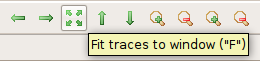
\includegraphics[scale=0.5]{./img/fittowindow.eps}
%    \end{center}
%    \caption{A population spike with multiple peaks (courtesy of Francisco Dubiela).}
%    \label{popspike}
%  \end{myfigure}
 
\subsection{Cutting traces to arbitrary lengths}
Cutting traces\keyindex{cuttingtraces}{traces!cutting}{trace cutting} is best
done using the squared bracket index operators (\pycommand{[]}) to slice a NumPy array. For example, if you wanted to cut a trace at the 100th sampling point, you could do:
\begin{lstlisting}
>>> a = get_trace()
>>> new_window(a[:100])
>>> new_window(a[100:])
\end{lstlisting}
In this example, \pycommand{a[:100]} refers to a sliced NumPy array that comprises all sampling points from index 0 to index 99, and \pycommand{a[100:]} refers to an array from index 100 to the last sampling point. \smallskip \\
\pycommand{\textbf{cut\_traces(pt)}}\pyindex{cuttraces}{cut\_traces}\\
\pycommand{\textbf{cut\_traces\_multi(pt\_list)}}\pyindex{cuttracesmulti}{cut\_traces\_multi}\\
These functions cut all selected traces at a single sampling point (\pycommand{pt}) or at multiple sampling points (\pycommand{pt\_list}). The cut traces will be shown in a new window. Both functions are included in the \pycommand{stf} namespace from version 0.8.11 on. The code for \pycommand{cut\_traces} is shown in listing \ref{cuttraceslisting}.
\begin{listing}
\lstset{numbers=left}
\begin{lstlisting}
import stf
import numpy as N

def cut_traces( pt ):
    """Cuts the selected traces at the sampling point pt,
    and shows the cut traces in a new window.
    Returns True upon success, False upon failure."""

    # Check whether anything has been selected:
    if not stf.get_selected_indices():
        return False
    new_list = list()
    for n in stf.get_selected_indices():
        if not stf.set_trace(n): return False

        # Check for out of range:
        if pt < stf.get_size_trace():
            new_list.append( stf.get_trace()[:pt] )
            new_list.append( stf.get_trace()[pt:] )
        else:
            print "Cutting point", pt, "is out of range"

    # Don't create a new window if everything was out of
    # range
    if len(new_list) > 0: stf.new_window_list( new_list )

    return True
\end{lstlisting}
\lstset{numbers=none}
  \caption {
    \pycommand{cut\_traces}
  }
  \label{cuttraceslisting}
\end{listing}
For example,
\begin{lstlisting}
>>> cut_traces_multi([100,900])
\end{lstlisting}
will cut all selected traces at sampling points 100 and 900 and show the cut traces in a new window. Note that you can pass a list or a tuple as an argument.
\begin{lstlisting}
>>> cut_traces_multi(range(100,2000,100))
\end{lstlisting}
will cut the selected traces at every 100th sampling point, starting with the 100th and ending with the 1900th (see p. \pageref{range} for the syntax of the \pycommand{range} function).


\chapter{Latency measurements}

\label{latencies}
\section{Measurement of synaptic delay}
Stimfit is frequently used to measure the \keyindex{synapticdelay}{synaptic delay}{synaptic delay}delay between a presynaptic signal and a postsynaptic response. Classically, this synaptic delay or \index{latency}latency is defined as ``the time interval between peak of inward current through the presynaptic membrane and commencement of inward current through the postsynaptic membrane'' \cite{Katz65}. Neglecting cable properties of neurons for a while, the maximal inward current during an action potential is expected to flow at the time of maximal slope during the rising phase \cite{Jack83}, since
\begin{align*}
  &I_\text{m}=I_\text{cap}+I_\text{ionic}=C_\text{m}\frac{\text{d}V_\text{m}}{\text{d}t}+I_\text{ionic}=0\text{,~and~hence}\\
  &I_\text{ionic}=-I_\text{cap}=-C_\text{m}\frac{\text{d}V_\text{m}}{\text{d}t}
\end{align*}
The commencement \keyindex{foot}{foot}{foot}(sometimes called ``foot'') of the postsynaptic current can robustly be estimated from the extrapolated intersection of the baseline with a line through the two points of time when the current is 20 and 80\% of the peak current (\citetext{Jonas93,Bartos01}; Fig. \ref{epscfoot}).
  \begin{myfigure}[htb]
    \begin{center}
      \input{img/foot}
    \end{center}
    \caption{Foot of an EPSC (red circle), estimated from the extrapolated intersection of the baseline with a line through the two points of time when the current is 20 and 80\% of the peak current (black open circles).}
    \label{epscfoot}
  \end{myfigure}

Although the method described above yields reliable results when both the pre- and the postsynaptic whole-cell recording show little noise and few artefacts, it may sometimes be favourable to use other estimates for the pre- and postsynaptic signals, for example when extracellular stimulation was used or when there are a lot of failures in the postsynaptic response. The following sections will explain how this is done in practice.

\section{Trace alignment}
It may sometimes be useful to \keyindex{tracealignment}{traces!alignment}{trace alignment}align traces before measuring the latency, either for visualisation purposes or to create an average without temporal jitter. Although an aligned average can be created using a toolbar button, the recommended way to align traces is to use the Python shell. \smallskip \\
\pycommand{\textbf{align\_selected(alignment, active=False)}}\pyindex{alignselected}{align\_selected}\\
This function aligns the selected traces to a point that is determined by the user-supplied function \pycommand{alignment} and then shows the aligned traces in a new window. The \pycommand{alignment} function is applied to the active channel if \pycommand{active=True} or to the inactive channel if \pycommand{active=False}. The alignment function has to return an index within a trace, and it should adhere to the general form \pycommand{index(active)}, where \pycommand{active} is a boolean indicating whether the active or the inactive channel should be used. The most common alignment functions are built into the program: \smallskip \\
\pycommand{\textbf{maxrise\_index(active)}}\pyindex{maxriseindex}{maxrise\_index}\\
\noindent returns the zero-based index of the maximal slope of rise in units of sampling points (see Fig. \ref{overview}), interpolated between adjacent sampling points, or a negative value upon failure.\smallskip\\
\pycommand{\textbf{peak\_index(active)}}\pyindex{peakindex}{peak\_index}\\
\noindent returns the zero-based index of the peak value in units of sampling points (see Fig. \ref{overview}), or a negative value upon failure. The return value may be interpolated if a moving average is used for the peak calculation (see p. \pageref{peakmovingaverage}).\smallskip\\
\pycommand{\textbf{foot\_index(active)}}\pyindex{footindex}{foot\_index}\\
\noindent returns the zero-based index of the foot of an event, as described on p. \pageref{foot} and in Fig. \ref{epscfoot}, or a negative value upon failure.\smallskip\\
\pycommand{\textbf{t50left\_index(active)}}\pyindex{t50leftindex}{t50left\_index}\\
\noindent returns the zero-based index of the left half-maximal amplitude in units of sampling points (see Fig. \ref{overview}), or a negative value upon failure. The return value will be interpolated between sampling points.\smallskip\\
\pycommand{\textbf{t50right\_index(active)}}\pyindex{t50rightindex}{t50right\_index}\\
\noindent  returns the zero-based index of the right half-maximal amplitude in units of sampling points (see Fig. \ref{overview}), or a negative value upon failure. The return value will be interpolated between sampling points.\smallskip\\
Listing \ref{alignall} shows a function that can be used to align all traces within a file to the maximal slope of rise in the inactive channel:
\begin{listing}
\lstset{numbers=left}
\begin{lstlisting}
# import the stimfit core module:
import stf

def align_maxrise():
    """Aligns all traces to the maximal slope of rise 
    of the inactive channel. Baseline and peak cursors
    have to be set appropriately before using this
    function.
    
    Return value:
    True upon success, False otherwise."""
    
    stf.select_all()
    
    # check whether there is an inactive channel at all:
    if ( stf.maxrise_index( False ) < 0 ):
        print "File not open, or no second channel; \
               aborting now"
        return False
        
    stf.align_selected( stf.maxrise_index, False )
    return True

\end{lstlisting}
\lstset{numbers=none}
  \caption {
    \pycommand{align\_maxrise}
  }
  \label{alignall}
\end{listing}

\section{Setting the latency cursors}
The \keyindex{latencycursors}{latency!cursors}{latency cursors}latency cursors (plottes as dotted vertical blue lines) can either be set automatically to some predefined points within a trace, or manually using the mouse buttons. The predefined points can be chosen from the menu: ``Edit''$\rightarrow$``Measure latency from...'' and ``Edit''$\rightarrow$``Measure latency to...''. The ``beginning'' of an event refers to the foot as explained above (Fig. \ref{epscfoot}). If ``Manually'' is selected, the left and right mouse buttons can be used to set the first and second latency cursors while the latency mode is activated. To switch to the latency mode, you can either click the corresponding button in the toolbar (Fig. \ref{latencybutton}) or press \keybox{L}.
  \begin{myfigure}[ht]
    \begin{center}
      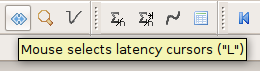
\includegraphics[scale = 0.5]{./img/latency.eps}
    \end{center}
    \caption{Activate latency mode.}
    \label{latencybutton}
  \end{myfigure}
  
To confirm your latency cursor settings and measure latencies, you can either press \keybox{Enter} or call \pycommand{measure()} from the shell (see p. \pageref{measure}). The latency, i.e. the time interval between the first and the second latency cursor, will be shown in the results table as long as you activated this value (see p. \pageref{resultstable}). The latency will be indicated as a double-headed arrow connecting the two latency cursors (Fig. \ref{latencytraces}).
  \begin{myfigure}[ht]
    \begin{center}
      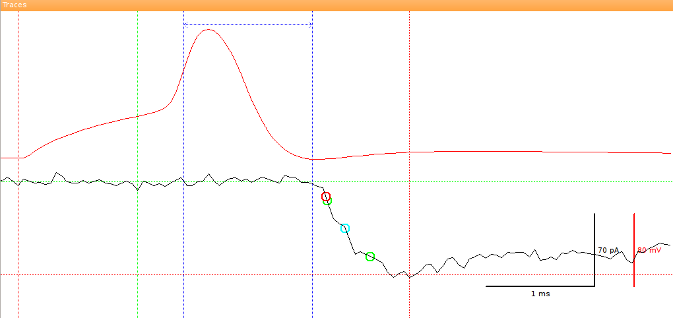
\includegraphics[scale = 0.4]{./img/latencytraces.eps}
    \end{center}
    \caption{The latency between the maximal slope of rise of an action potential (red) and the foot of an EPSC (black) is indicated by a horizontal double-headed arrow.}
    \label{latencytraces}
  \end{myfigure}


\chapter{Event extraction by template matching}

\label{extractevents}
\section{Introduction}
To isolate individual events such as EPSCs or EPSPs from recorded data, Stimfit uses a\keyindex{templatematching}{event detection!template matching}{template matching}\index{template matching|see{event detection}} template matching algorithm as decribed by \citetext{Jonas93}, with some implementation details adopted from \citetext{Clements97}. The template consists of a waveform $p(t)$ with a length of $n$ sampling points that represents the time course of a typical event. The template is slid over the trace of recorded values $r(t)$, and at each sampling point with index $s$, it is multiplied by a scaling factor $m$ and an offset $c$ is added or subtracted so that the sum of squared errors $\chi^2(t_s)$ between the trace and the template is minimised:
\begin{equation*}
  \chi^2(t_s)=\sum_{k=0}^{n-1}\left[r(t_{s+k})-\left(m{\cdot}p(t_k)+c\right)\right]^2
\end{equation*}
As can be seen from this equation, this amounts to the fairly simple operation of fitting a straight line that relates $p(t)$ and $r(t)$ at every sampling point.

Finally, some \keyindex{detectioncriterion}{event detection!detection criterion}{detection criterion}\index{detection criterion|see{event detection}}detection criterion has to be applied to decide whether an event has occurred at a sampling point. Two options are available in Stimfit: \citetext{Jonas93} suggest to use the linear correlation coefficient between the optimally scaled template and the data, whereas \citetext{Clements97} compare the scaling factor with the noise standard deviation.

\section{A practical guide to event detection}
In practice, the following steps need to be performed to extract events with Stimfit:
\begin{enumerate}
 \item Create a preliminary template by fitting a function to a single, large and isolated event.
 \item Use this preliminary template to extract some more examplary large and isolated events using a high detection criterion threshold.
 \item Create the final template by fitting a function to the average of the exemplary events.
 \item Extract all events with the final template using a low detection criterion threshold.
 \item Eliminate false-positive, add false-negative events.
\end{enumerate}
This procedure will be explained in some more detail in the following sections.

\subsection{Create a preliminary template}
In general, the template waveform $p(t)$ can be of arbitrary shape. A typical way of creating such a template is to fit a function with a time course matching the event kinetics to some exemplary events. For example, EPSCs can typically be modelled with the sum or the product of two exponential functions \footnote{Note that the product of two exponentials $f(t)=a\left(1-e^{-\frac{t}{\tau_1}}\right)e^{-\frac{t}{\tau_2}}$ can equivalently be expressed as the sum of two exponentials: $f(t)=a\left(e^{-\frac{t}{\tau_2}}-e^{-\frac{t}{\tau_3}}\right)$, with $\tau_3=\frac{\tau_1\tau_2}{\tau_2-\tau_1}$.}. In practice, a robust estimate for a template can be obtained using an iterative approach, which will be illustrated here using a recording of miniature EPSCs that you can download \href{http://stimfit.org/tutorial/minis.dat}{here}\footnote{\url{http://stimfit.org/tutorial/minis.dat}}.

\label{bait}First, we fit a function to a single large and isolated event to create a preliminary ``bait'' template.
  \begin{myfigure}[htb]
    \begin{center}
      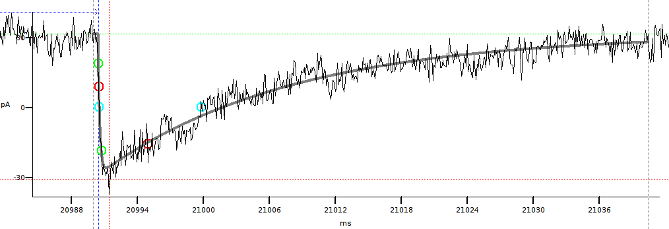
\includegraphics[scale=0.41]{./img/bait_template.eps}
    \end{center}
    \caption{Creation of a ``bait'' template.}
    \label{baittemplate}
  \end{myfigure}
In this case, we will use the EPSC that can be found roughly between \textit{t}~=~20990~ms and \textit{t}~=~21050~ms. Then, we fit the sum of two exponential functions with a delay to this EPSC. To obtain the same template as in the example, you can call the function \pycommand{preliminary} from the \pycommand{minidemo} module that comes bundled with stimfit:
\begin{lstlisting}
>>> import minidemo
>>> minidemo.preliminary()
\end{lstlisting}
This will take care of the appropriate cursor positions and the biexponential fit (see p. \pageref{setpeakstart} for setting the cursors from Python, and p. \pageref{leastsq} for the \pycommand{leastsq} function). If you prefer, you can use the fit settings dialog as described in chapter \ref{gettingstarted} (Fig. \ref{fitselection}, p. \pageref{fitselection}).

\subsection{Extract exemplary events}
We now use the bait template to fish some more large and isolated events. Choose ``Analysis''$\rightarrow$``Event detection'' $\rightarrow$``Template matching...'' from the menu.
  \begin{myfigure}[htb]
    \begin{center}
      \includegraphics[scale=0.5]{./img/event_dialog.eps}
    \end{center}
    \caption{Event detection settings.}
    \label{eventdialog}
  \end{myfigure}
In the dialog that will pop up (Fig. \ref{eventdialog}), you can set the threshold for the detection criterion. Since we want to extract some large and isolated events during this first pass, we set this to a high number, say 10, using the template scaling factor \cite{Clements97}. Click ``OK'' to start the event detection. When finished, press \keybox{F} to fit the whole trace to the window. The detected events will be marked by blue arrows in the upper part of the window, and blue circles will indicate the peak values of the detected events (Fig. \ref{events}).
  \begin{myfigure}[htb]
    \begin{center}
      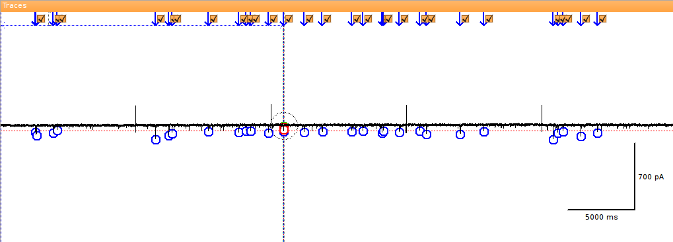
\includegraphics[scale=0.4]{./img/events.eps}
    \end{center}
    \caption{Detected events.}
    \label{events}
  \end{myfigure}
To view the isolated events in a new window, you have to switch to the event editing mode, either by pressing \keybox{E} or by activating the corresponding button in the toolbar (Fig. \ref{eventbutton}).
  \begin{myfigure}[htb]
    \begin{center}
      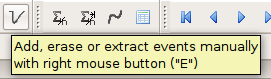
\includegraphics[scale=0.5]{./img/eventbutton.eps}
    \end{center}
    \caption{Switching to event editing mode.}
    \label{eventbutton}
  \end{myfigure}
When you now click on the trace with the right mouse button, a menu will show up. Select ``Extract selected events'' from this menu. This will put the exemplary EPSCs into a new window.

\subsection{Create the final template}
We now create the average of all extracted events, as explained in chapter \ref{gettingstarted} (p. \pageref{averagecalculation}). Then, we fit a biexponential function to the average, as explained above for the single EPSC (see p. \pageref{bait}). Remember to set the baseline, peak and fit window cursors appropriately before performing the fit, and to update all calculations. Again, you can make use of a function from the \pycommand{minidemo} module to set the cursors and perform the fit:
\begin{lstlisting}
>>> import minidemo # if you haven't imported it already
>>> minidemo.final()
\end{lstlisting}
The final template should look similar as shown in Fig. \ref{finaltemplate}.
  \begin{myfigure}[htb]
    \begin{center}
      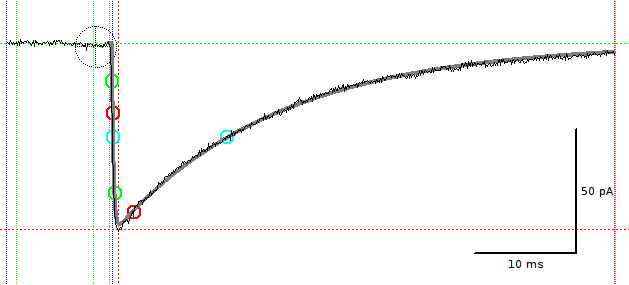
\includegraphics[scale=0.5]{./img/finaltemplate.eps}
    \end{center}
    \caption{Creating a final template.}
    \label{finaltemplate}
  \end{myfigure}

\subsection{Extract all events}
Go back to the original file (minis.dat). Extracting all events with the final template is done in nearly the same way as described above for the preliminary template. However, you have to choose the correct template in the event dialog: The final template in this case is the second on the list (Fig. \ref{selectfinal}).
  \begin{myfigure}[htb]
    \begin{center}
      \includegraphics[scale=0.5]{./img/selectfinal.eps}
    \end{center}
    \caption{Selecting the final template.}
    \label{selectfinal}
  \end{myfigure}
For this final run, we will lower the detection threshold to a value of 3, as suggested by \citetext{Clements97}.

\subsection{Edit detected events}
Usually, the detected events have to be screened visually to remove false-positives and add false-negatives. Removing false positives is done by unselecting the checkbox next to the arrow indicating an event (Fig. \ref{events}). To add false-negatives, you have to switch to the event-editing mode (Fig. \ref{eventbutton}) and then right-click on the trace at the position where the event starts. From the context menu that will pop up, select ``Add an event that starts here'' (Fig. \ref{falsenegative}). To efficiently screen the whole trace, it is convenient to use \keybox{Shift} and \keybox{$\leftarrow$} at the same time. This will move the trace left by the width of one window. Once you are done with editing, choose ``Extract selected events'' from the context menu.
  \begin{myfigure}[htb]
    \begin{center}
      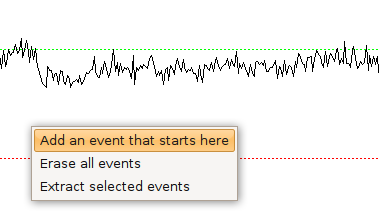
\includegraphics[scale=0.5]{./img/falsenegative.eps}
    \end{center}
    \caption{Adding a false-negative event.}
    \label{falsenegative}
  \end{myfigure}

\subsection{Analyse extracted events}
If you used the same settings as suggested above, 97 events will be extracted. You will find a table on the left of the traces: This will show you the time of onset of the events and the inter-event intervals. Usually, you will want to apply some further analysis to the extracted events. To do so, you first have to adjust the baseline, peak and fit cursors. Again, there is a function in the \pycommand{minidemo} module taking care of that:
\begin{lstlisting}
>>> minidemo.batch_cursors()
\end{lstlisting}
To analyse all traces efficiently, you can now perform a \keyindex{batchanalysis}{batch analysis}{batch analysis}``batch analysis'' on all traces at once: First, select all traces, either using \pycommand{select\_all()} from the shell (see p. \pageref{selectall}) or ``Edit''$\rightarrow$``Select all traces'' from the menu or pressing \keybox{Ctrl} and \keybox{A} at the same time. Then, choose ``Analysis''$\rightarrow$``Batch analysis'' from the menu.
  \begin{myfigure}[htb]
    \begin{center}
      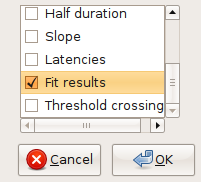
\includegraphics[scale=0.5]{./img/batchanalysis.eps}
    \end{center}
    \caption{Batch analysis settings.}
    \label{batchanalysisdlg}
  \end{myfigure}
From the dialog (Fig. \ref{batchanalysisdlg}), choose the analysis functions that you want to apply to your data. Click ``OK'' once you are done. A new table will appear to the left of the traces. You can copy and paste values from the tables to spreadsheet programs for further analysis.

\subsection{Adjusting event detection settings}
\small
\begin{tabular}{p{0.45\textwidth} p{0.45\textwidth}}
\textit{Problem} & \textit{Solution} \\ \hline 
 & \\
Too many false-positive events have been detected & Increase the detection threshold \\
 & \\
Too many events have been missed (false-negatives) & Decrease the detection threshold \\
 & \\
One and the same event is detected multiple times at short time intervals & Increase the number of sampling points between events \\
 & \\
Closely spaced events are not detected separately & Decrease the number of sampling points between events \\
\end{tabular}


\backmatter

\chapter{Keyboard shortcuts}

\label{shortcuts}\index{shortcuts|see{keyboard shortcuts}}\index{keyboard shortcuts}
\scriptsize
\begin{tabular}{l l p{0.61\textwidth}}
\textbf{Key}           & \textbf{Action}        & \smallskip \\
\keybox{B}             & \textit{followed by}   & \,               \\
\,                     & left mouse button      & Sets left cursor (lower limit) of baseline window \\
\,                     & right mouse button     & Sets right cursor (upper limit) of baseline window \\
\keybox{D}             & \textit{followed by}   & \,               \\
\,                     & left mouse button      & Sets left cursor (lower limit) of fit window \\
\,                     & right mouse button     & Sets right cursor (upper limit) of fit window \\
\keybox{E}             & \textit{followed by}   & \,               \\
\,                     & right mouse button     & Pops up a context menu for event editing\\
\keybox{L}             & \textit{followed by}   & \,               \\
\,                     & left mouse button      & Sets the left latency cursor \\
\,                     & right mouse button     & Sets the right latency cursor \\
\keybox{P}             & \textit{followed by}   & \,               \\
\,                     & left mouse button      & Sets left cursor (lower limit) of peak window \\
\,                     & right mouse button     & Sets right cursor (upper limit) of peak window \\
\keybox{Z}             & \textit{followed by}   & \,               \\
\,                     & left mouse button      & Drag a window around the region you want to zoom in \\
\,                     & right mouse button     & Choose action from context menu \medskip \\
\keybox{Enter}         & \multicolumn{2}{l}{Measure peak, baseline and latency, update results table} \medskip \\
\keybox{1}             & \multicolumn{2}{l}{Scaling operations apply to the active (black) channel} \\
\keybox{2}             & \multicolumn{2}{l}{Scaling operations apply to the inactive (red) channel} \\
\keybox{3}             & \multicolumn{2}{l}{Scaling operations apply to both channels} \medskip \\
\keybox{$\uparrow$}    & \multicolumn{2}{l}{Shift traces up} \\
\keybox{$\downarrow$}  & \multicolumn{2}{l}{Shift traces down} \\
\keybox{$\leftarrow$}  & \multicolumn{2}{l}{Previous trace} \\
\keybox{$\rightarrow$} & \multicolumn{2}{l}{Next trace} \\
\keybox{+}             & \multicolumn{2}{l}{Enlarge traces vertically} \\
\keybox{-}             & \multicolumn{2}{l}{Shrink traces vertically} \medskip \\
\keybox{S}             & \multicolumn{2}{l}{Select the currently displayed trace} \\
\keybox{R}             & \multicolumn{2}{l}{Remove the currently displayed trace from the stack of selected traces} \medskip \\
\keybox{Ctrl}          & \textit{together with} & \,               \\
\,                     & \keybox{+}             & Enlarge traces horizontally \\
\,                     & \keybox{-}             & Shrink traces horizontally \\
\,                     & \keybox{$\leftarrow$}  & Shift traces left \\
\,                     & \keybox{$\rightarrow$} & Shift traces right \\
\,                     & \keybox{A}             & Select all traces \medskip \\
\keybox{Shift}         & \textit{together with} & \,               \\
\,                     & \keybox{$\leftarrow$}  & Shift traces left by one window width \\
\,                     & \keybox{$\rightarrow$} & Shift traces right by one window width \\

\end{tabular}
\normalsize

% \renewcommand\refname{}
% \begin{multicols}{2}
% \setlength\columnseprule{.3pt}
% \footnotesize
\bibliography{/home/cs/doc/bib/all}
% \normalsize
% \end{multicols}

\footnotesize
\printindex
\normalsize

\end{document}
